\documentclass[10pt,twocolumn]{article}

% Följande rad ska göra det möjligt att använda svenska bokstäver, som å, ä, ö. Kravet är 
% då att filen sparas i UTF-8-format. Om detta inte fungerar för dig, så kan du alltid 
% använda dig av {\aa} för å, \"a för ä och \"o för ö.
\usepackage[utf8]{inputenc}

% Följande väljer typsnitt som är kloner av Times New Roman, Helvetica och lämpliga till
% dem anpassade matematiktypsnitt.
\usepackage{newtxtext}
\usepackage{newtxmath}

%  Följande tillhandahåller miljön spver­ba­tim som är lämplig för att typsätta programkod.
\usepackage{spverbatim}
\usepackage{graphicx}

\renewcommand{\figurename}{Figur}

\raggedbottom
\sloppy

\title{Laborationsrapport i TSKS10 \emph{Signaler, Information och Kommunikation}}

\author{Malcolm Vigren \\ malvi108, 19950127-0970 }

\date{xxx maj, 2017}

\begin{document}

\maketitle

\section{Inledning}

Syftet med denna laboration var att IQ-demodulera och behandla en radiosignal
för att kunna höra vad som sändes. Enligt problemformuleringen skickar
radiostationen signalen:
\begin{align*}
    x(t) = x_I(t)\cos(2 \pi f_c t) - x_Q(t)\sin(2 \pi f_c t) + w(t) + z(t)
\end{align*}
där $x_Q(t)$ och $x_I(t)$ är de meddelanden som skulle lyssnas efter. De
innehåller båda två olika melodier samt varsitt ordspråk som ska identifieras.
$f_c$ är signalens bärfrekvens, $z(t)$ är en summa av andra I/Q-modulerade
signaler och $w(t) = 0.001(\cos(2 \pi f_1 t) + \cos(2 \pi))$, där $f_1$ och
$f_2$ ligger långt ifrån bärfrekvenserna hos de andra signalerna. En del av
uppgiften är att ta reda på $f_c$, $f_1$ och $f_2$. $f_c$ var enligt
problemformuleringen en av följande frekvenser: 18, 37, 56, 75, 94, 113,
132, 151 kHz.

På grund av utformningen hos miljön innehåller den mottagna signalen en
ekoeffekt, sådan att vi tar emot signalen:
\begin{align*}
    y(t) = x(t - \tau_1) + 0.9x(t - \tau_2)
\end{align*}
En del av uppgiften är att ta reda på fördröjningen mellan de olika signalerna,
alltså $\tau_2 - \tau_1$. Denna är enligt problemformuleringen mindre än 500 ms
och en multipel av 1 ms.

Signalen är sparad i en \textit{wav}-fil med sampelfrekvensen 400kHz.

\section{Metod}

Detta avsnitt redogör hur den efterfrågade informationen togs fram.

\subsection{Letande av kandidater till $f_c$ och bestämmande av $f_1$ och
$f_2$}

För att ta reda på $f_c$ fouriertransformerades signalen i wav-filen, och
amplitudspektrumet plottades, se Figur~\ref{fig:yamp}. 
\begin{figure}[h]
    \centering
    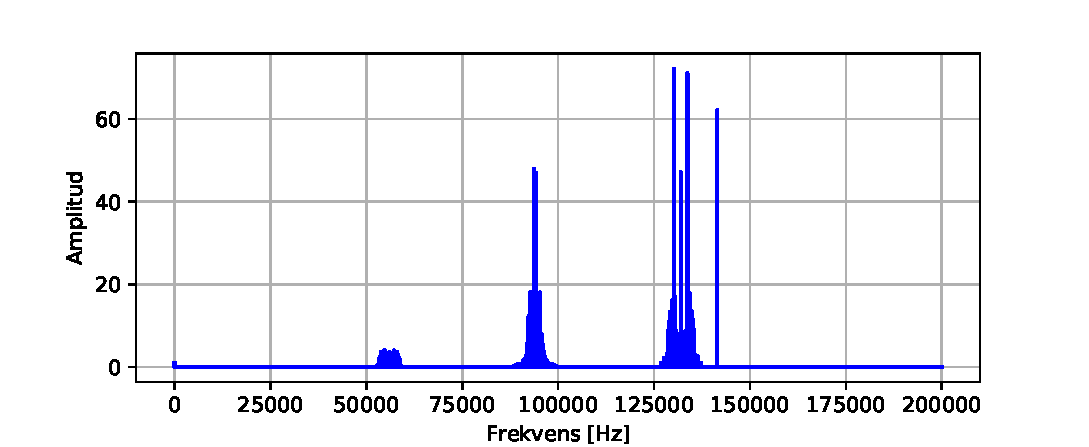
\includegraphics[width=\linewidth]{figures/yamp.pdf}
    \caption{Amplitudspektrum för $y(t)$}
    \label{fig:yamp}
\end{figure}
Från detta kunde den del kandidater till $f_c$ uteslutas, sådan att
de möjliga värdena var 56, 94, 132 kHz, då det är runt dessa frekvenser de
olika signalerna samlas runt. Från detta kan också frekvenserna för
cosinussignalerna från $w(t)$
bestämmas, då dessa är två mycket närliggande spikar vid 141500 respektive
141501 Hz. Alltså är $f_1=141500$ Hz och $f_2=141501$ Hz.

\subsection{I/Q-demodulering\label{sub:iq}}
För att demodulera signalen bandpassfiltrerades signalen för att extrahera
signalen för en viss frekvens. Detta gjordes genom att bestämma vilka
frekvensband varje signal befann sig i från Figur~\ref{fig:yamp}, och använda
ett digitalt butterworthfilter för att filtrera ut signalen. Den filtrerade
signalen multiplicerades med $2\cos(2\pi f_c t + \delta)$ och 
$-2\sin(2\pi f_c t + \delta)$ 
för att få ut $x_I(t)$- respektive $x_Q(t)$-komponenterna av signalen.
Konstanten $\delta$ finns som kompensation för fasvridningen signalen får efter
att den skickats, som sattes till en början till 0. Hur $\delta$ bestämdes
beskrivs i Avsnitt~\ref{sub:delta}. Båda
lågpassfiltrerades sedan med ett digitalt butterworthfilter med samma bandbredd
som signalerna för att filtrera
bort de frekvenser som fortfarande fanns runt bärvågsfrekvensen.

Detta gjordes som sagt för varje av de intressanta banden i $y(t)$ för att ta
reda på vilket band som innehöll det intressanta ljudet. Det visade sig att det
band med mittenfrekvens 94 kHz innehöll något som liknade beskrivningen av
ljudet i problemformuleringen. Därför drogs slutsatsen att $f_c = 94$ kHz.
Det noterades också att signalen med bärfrekvens 56 kHz innehöll en vågform som
liknande vitt brus.

\subsection{Bestämmande av $\tau_2 - \tau_1$}
För att bestämma fördröjningen $\tau_2 - \tau_1$ användes autokorrelation. För
att göra detta utnyttjades det faktum att ett $\tau_2$ sekunder in i signalen
hörs inget eko, vilket betyder att man kan använda signalen fram till $\tau_d$
sekunder som det som ska korreleras, där $\tau_d < \tau_2$.

Vi betecknar signalvärdet vid sampel $n$ som $y_n$. Vidare definierar vi korrelationen
$z(\tau)$ som:

\begin{equation*}
    z(\tau) = \frac{1}{f_s}\sum_{i=0}^{\tau_d}y_iy_{i + \tau f_s}
\end{equation*}

\subsection{Bestämmande av $\delta$\label{sub:delta}}

\section{Resultat}

Den sökta informationen är:
\begin{itemize}
\item Bärfrekvensen för nyttosignalen är $f_c=94$ kHz.
\item $f_1=141500$ Hz och $f_2=141501$ Hz
\item $\tau_2 - \tau_1 = 420$ ms.
\item Ordspråket i $x_I(t)$ är "Väck inte den björn som sover".
\item Ordspråket i $x_Q(t)$ är "Äpplet faller inte långt från trädet".
\end{itemize}

\clearpage

\section*{Min Matlab-kod:}
\begin{spverbatim}
clear all
close all

for k=1:...
  ...
end

plot(...,...)
\end{spverbatim}

\end{document}
